% !TEX root = ../main.tex

% ---------------------------------------------------------------
% Automatic generation of a self-adaptive TLM model
% ---------------------------------------------------------------

\chapter[Apprendimento non supervisionato]{Apprendimento non supervisionato per l'identificazione di contensti di FoG}\label{chap5:Automatic}
I lavori che sono stati svolti e presentati nel capitolo \ref{chap2:related} sul Freezing Of Gait sono basati principalmente sull'identificazione di 2 classi, ossia quando il paziente é in una normale attivitá quotidiana, che chiameremo NoFoG, oppure quando il paziente soffre di un episodio di FoG. Qualcuno di essi, invece, ha accennato alla possibile esistenza di una fase intemedia tra noFoG e FoG. Il nostro lavoro vuole dimostrare ed identificare tale nuova classe, che viene chiamata preFoG. Questa dovrebbe rappresentare la fase di transizione da uno stato di NoFoG ad uno di FoG, per cui identificare tale classe permetterebbe di anticipare l'occorrenza di un FoG e, quindi, dare in anticipo uno stimolo al paziente per evitare il verificarsi del FoG. La durata di ogni preFoG, nei lavori in cui è stata accennata la sua esistenza, viene fissata a due secondi, per cui noi vogliamo vedere se, con tale intervallo fissato, la classe è distinguibile effettivamente dalle altre. Il flusso della tesi viene rappresentato in figura \ref{FlussoTesi}.\\
\begin{figure}[]
	\centering
	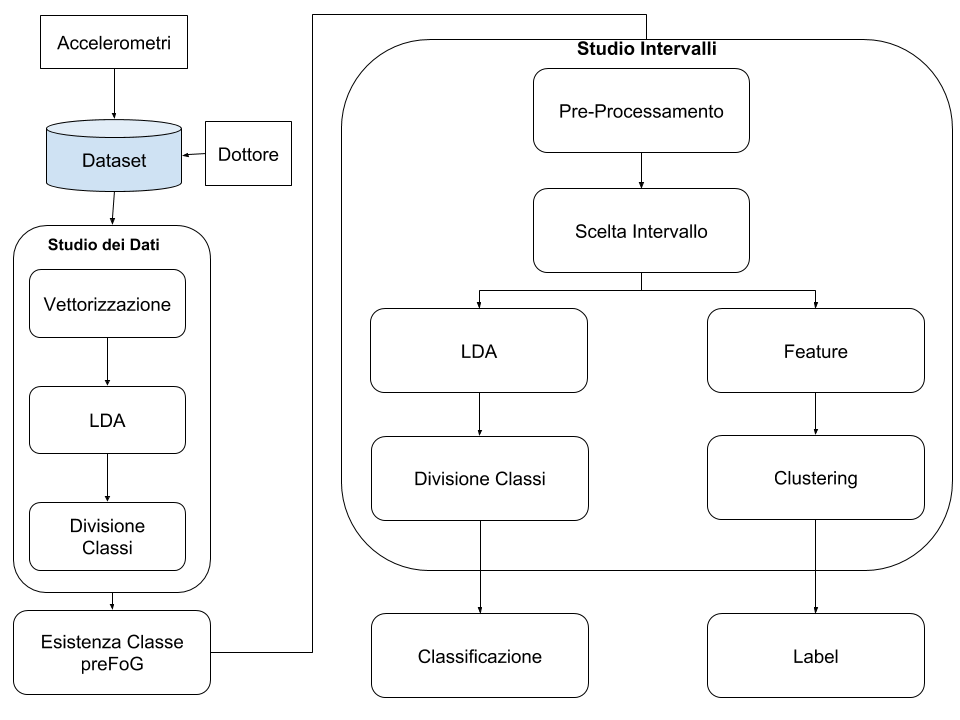
\includegraphics[scale=0.35]{images/FlussoTesi.png}
	\caption{Rappresentazione del flusso della tesi}
	\label{FlussoTesi}
\end{figure}
Lo sviluppo della procedura é stato svolto usando software Matlab.
\section{Dataset}
L'approccio che andiamo a proporre è stato testato sul dataset DAPHNET\footnote{www.wearable.ethz.ch/resources/Dataset}, il quale contiene dati collezionati da 10 pazienti parkinsoniani, dei quali 8 presentano contesti di FoG, mentre 2 di loro non ne presentano. I dati sono stati registrati usando 3 accelerometri 3D attaccati alla caviglia, al ginocchio e nella zona lombare del paziente, usando una frequenza di campionamento di 64 Hz, ossia vengono raccolti 64 campioni ogni secondo.\\
I soggetti hanno completato sessioni da 20-30 minuti ciascuno, consistenti di 3 fasi di camminata:
\begin{enumerate}
	\item Camminata avanti ed indietro lungo una linea retta, con delle rotazioni di 180 gradi;
	\item Camminata casuale con una serie di fermate volontarie e rotazioni di 360 gradi;
	\item Camminata che simula attività di vita quotidiana, tra le quali entrare in stanze ed uscirne, camminare nella cucina, prendersi un bicchiere d'acqua e tornare al punto di partenza.
\end{enumerate}
Le prestazioni motorie variano molto tra i pazienti. Mentre alcuni soggetti hanno mantenuto una camminata regolare durante gli episodi di non FoG, altri hanno camminato molto lentamente ed in modo instabile. L'intero dataset contiene in totale 237 episodi di FoG; la durata di ognuno di essi è tra i 0.5s ed i 40.5s. Il 50\% degli episodi di FoG è durato meno di 5.4s ed il 93.2\% è più corto di 20s. Gli episodi di FoG sono stati identificati da fisioterapisti usando registrazioni video sincronizzate. L'inizio di un episodio di FoG è stato definito come il punto dove la sequenza normale di camminata è stata interrotta, mentre la fine del FoG è stata definita come il momento in cui tale sequenza riprende.

\section{Dimostrazione dell'esistenza della classe preFoG}
Nel lavoro svolto in questa tesi si vogliono usare 3 classi invece delle 2 fornite dal dataset. Il primo passo dunque é quello di dimostrare che effettivamente le 3 classi sono distinte tra loro e che quindi sviluppare un approccio basandosi su tali classi é possibile.\\
Per fare questo, si é usato un approccio di Discriminazione Lineare. Un discriminante é una funzione che prende in ingresso un vettore x e lo assegna ad una tra le K classi fornite. Il metodo di discriminazione che si vuole usare é quello di Fisher, il quale viene spiegato nel Capitolo \ref{chap3:background}.\\
\subsection{Divisione dei dati}
Per ogni paziente, prendiamo in input la matrice di dati grezzi degli accelerometri fornita dal dataset, la quale contiene anche un campo relativo al tempo di ogni campione ed un'etichetta, che mi indica lo stato in cui si trova il mio paziente. Dividiamo i dati degli accelerometri da quelli relativi al tempo ed allo stato e calcoliamo delle feature su tali dati. Queste vengono calcolate vettorizzando finestre di dati grezzi, ossia prendendo tutte le righe e colonne della finestra e disponendole lungo un vettore riga.  Ogni nuova finestra non comincia dalla fine della precedente, ma presenta una certa sovrapposizione. Per tenere traccia dell'etichetta reale a cui ogni finestra temporale appartiene, abbiamo usato il vettore relativo all'etichetta fornita dal dataset e, per ogni finestra temporale, abbiamo tenuto quella che si presenta più volte all'interno di essa. Il codice implementativo di quanto appena descritto é fornito in \ref{vettorizzazione}.
\begin{lstlisting}[style=Matlab-editor,frame=single, caption=Vettorizzazione dei dati degli accelerometri, label=vettorizzazione]
for i=1:size_windows_sample-size_overlap_samples:m - size_windows_sample
B = A(i:i+size_windows_sample-1,:);
% vettorizzo ogni finestra
B=B(:);
F(number_sample,:)=B';


%salvo la classe di ogni finestra
class(number_sample)=mode(FREEZE(i:i+size_windows_sample-1,:));

%go to next sample
number_sample = number_sample + 1;

end
\end{lstlisting}
\subsection{Algoritmo di discriminazione}
Una volta vettorizzato l'intero dataset, si procede ad applicare l'algoritmo di discriminazione, il quale per prima cosa divide le feature appena calcolate tramite le classi di appartenenza. Calcola quindi la media per ogni classe e determina la dimensione di ognuna di esse. A questo punto, determina la within class covariance e la between class covariance, ossia quanta similaritá esiste tra gli elementi della stessa classe e quanta dissimilaritá é presente tra classi differenti. Una volta trovate tali misure, prende gli autovalori ed autovettori della soluzione del problema dell'autovalore generalizzato e tiene solo quelli più rappresentativi, che nel caso dell'approccio di Fisher sono pari al numero di classi presenti meno 1. Questi autovalori vengono poi moltiplicati per le feature calcolate precedentemente per ottenere una riduzione della dimensionalità' ed avere 2 feature rappresentative. Il codice della discriminazione viene fornito in \ref{code_LDA}.
\begin{lstlisting}[style=Matlab-editor,frame=single, caption=LDA, label=code_LDA]
A=F';

%quindi ho A 1152x1449 double
%1152 finestre
%ogni finestra ha 1449 features
[d,N] = size(A);

K =  max(class); % numero classi in gioco;

% 1. Divido le feature tramite le classi Ck
for k = 1:K
a = find (class == k);
Ck{k} = A(:, a);
end

% 2. Calcolo la media per ogni classe per ogni finestra
for k = 1:K
mk{k} = mean(Ck{k},2);
end
% 3. Determino la grandezza di ogni classe
for k = 1:K
[d, Nk(k)] = size(Ck{k});
end
% 4. determino le within class covariance
for k = 1:K
S{k} = 0;
for i = 1:Nk(k)
S{k} = S{k} + (Ck{k}(:,i)-mk{k})*(Ck{k}(:,i)-mk{k})';
end
S{k} = S{k}./Nk(k);
end
Swx = 0;
for k = 1:K
Swx = Swx + S{k};
end

% 5. determino la between class covariance
% 5.1 determino la media totale
m = mean(A,2);
Sbx = 0;
for k=1:K
Sbx = Sbx + Nk(k)*((mk{k} - m)*(mk{k} - m)');
end
Sbx = Sbx/K;

MA = inv(Swx)*Sbx;

% eigenvalues/eigenvectors
[V,D] = eig(MA);

% 5: transform matrix
if (k > 1)
W = V(:,1:K-1);
end
if (k == 1)
W = V(:,1:1);
end

% 6: transformation
Y = W'*A;
\end{lstlisting}
\subsection{Risultati}
Una volta calcolate le feature discriminanti, per visualizzare se effettivamente c'é una distinzione tra le classi, facciamo un grafico con queste due grandezze ed ogni punto viene colorato in base alla reale classe di appartenenza.\\
Le figura \ref{LDAS01} e \ref{LDAS02} fanno notare immediatamente come le feature utilizzate riescono a discriminare abbastanza tra le 3 classi, anche se c'è ancora una certa sovrapposizione tra i dati di classi diverse, prendendo i dati di un solo paziente.\\
Ogni soggetto, però, ha dei pattern di camminata diversi, quindi posso avere dati molto differenti tra un paziente ed un altro. Abbiamo quindi verificato anche se, utilizzando i dati di tutti i pazienti, la discriminazione lineare riesce ancora a distinguere in modo più o meno buono.\\
La figura \ref{LDAALL} mostra, che prendendo i dati di tutti i pazienti assieme, una certa divisione rimane, anche se è molto meno netta rispetto al singolo paziente. Questo comunque ci permette di dire che anche tra pazienti differenti, quindi con pattern di cammino diversi, i dati che sono di preFoG sono abbastanza divisi da quelli di noFoG o FoG, quindi un approccio concentrato su questa nuova classe sembra sensato.

\begin{figure}[]
	\centering
	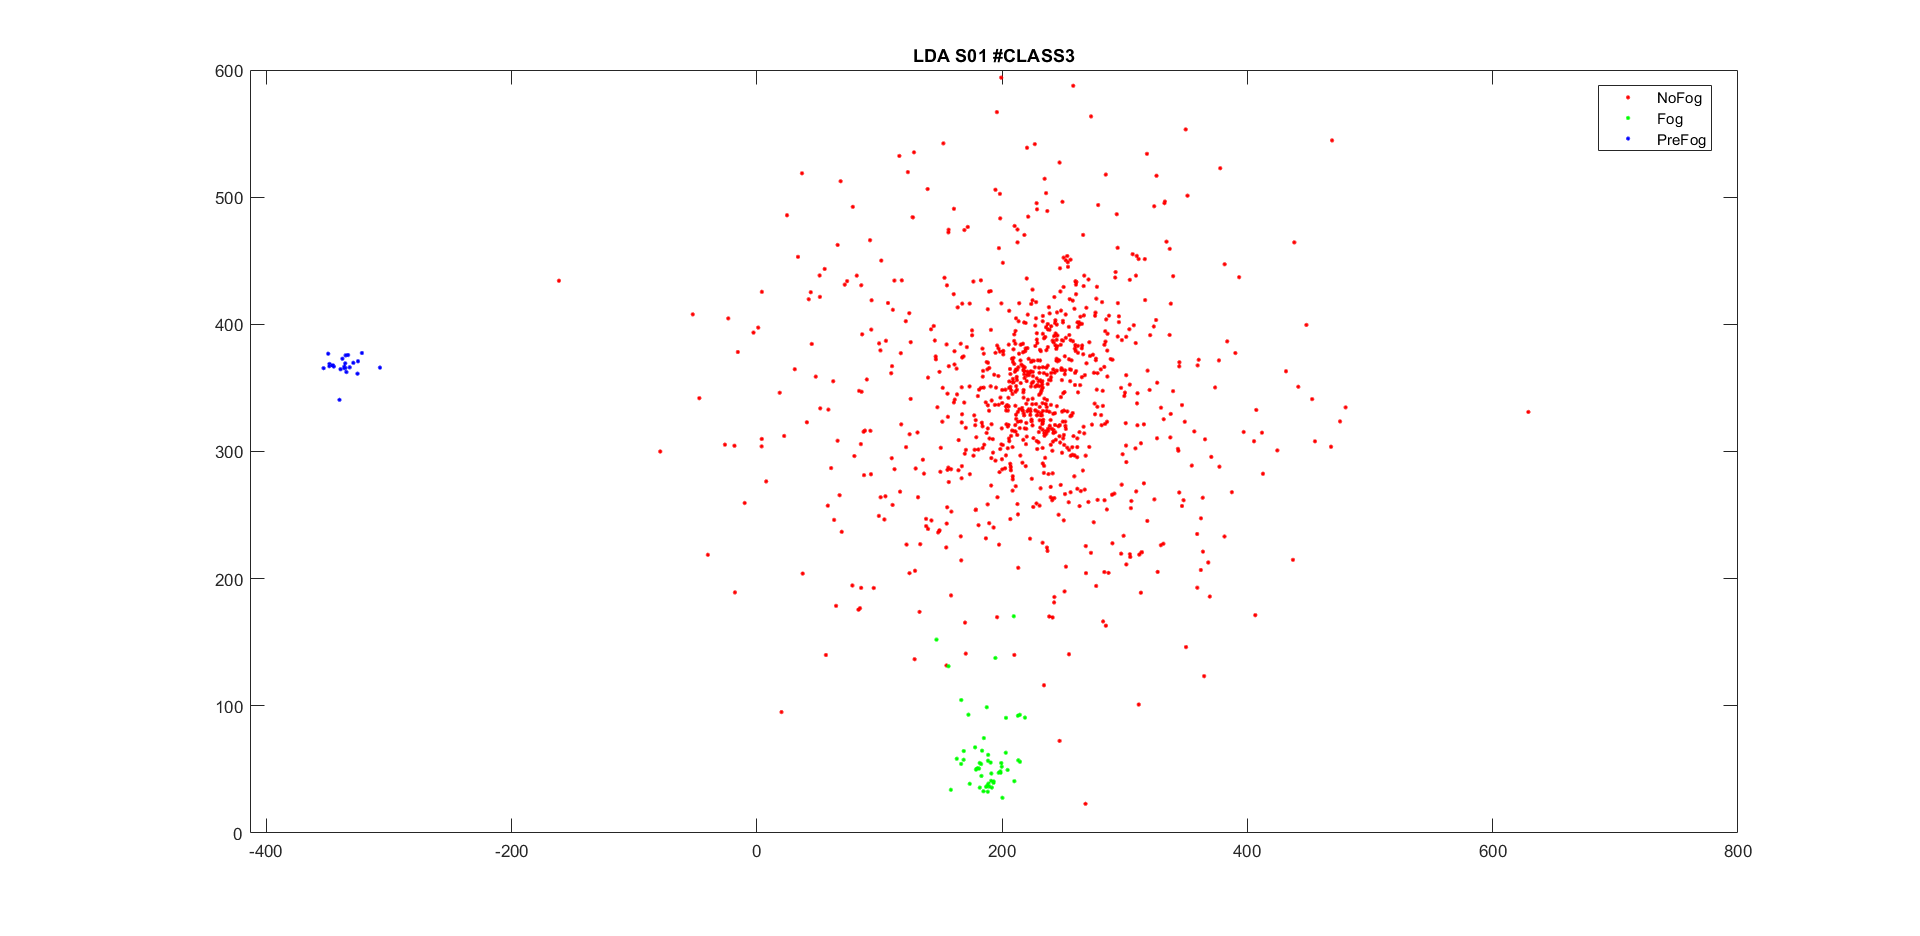
\includegraphics[scale=0.25]{images/LDAS01.png}
	\caption{Grafico delle 3 classi in base alla discriminazione dell'approccio di Fisher per il paziente 1}
	\label{LDAS01}
\end{figure}
\begin{figure}[]
	\centering
	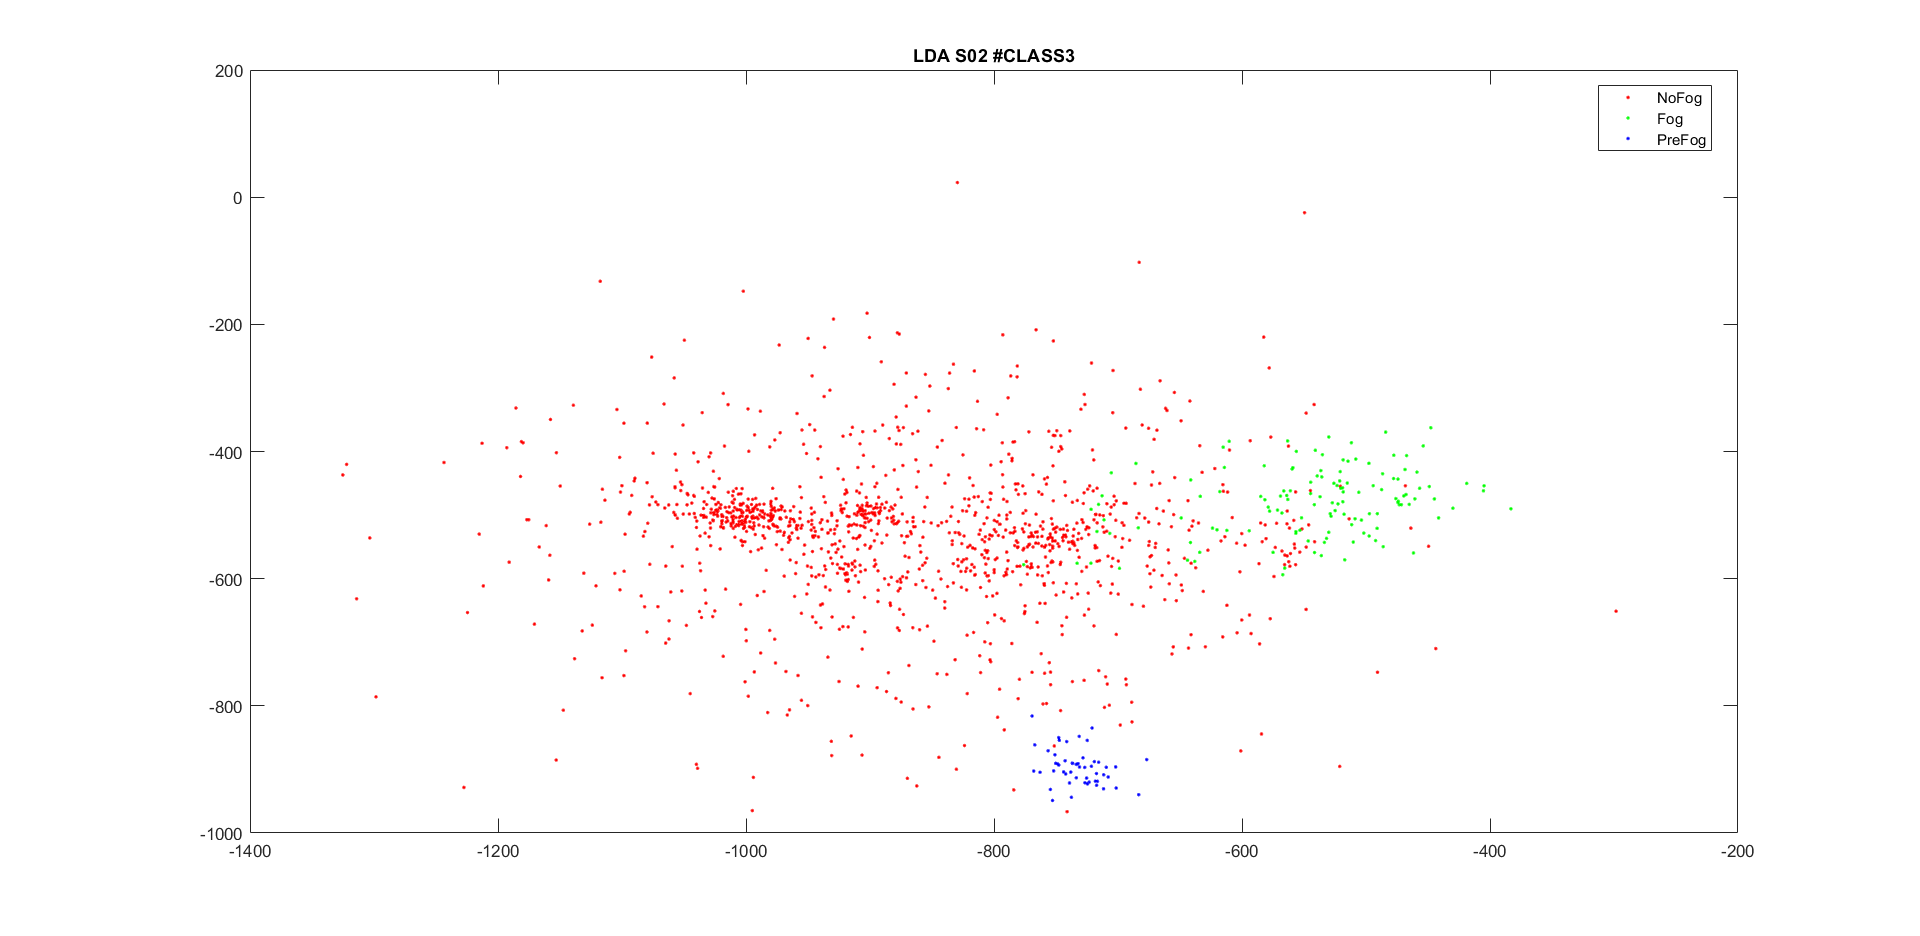
\includegraphics[scale=0.25]{images/LDAS02.png}
	\caption{Grafico delle 3 classi in base alla discriminazione dell'approccio di Fisher per il paziente 2}
	\label{LDAS02}
\end{figure}
\begin{figure}[]
	\centering
	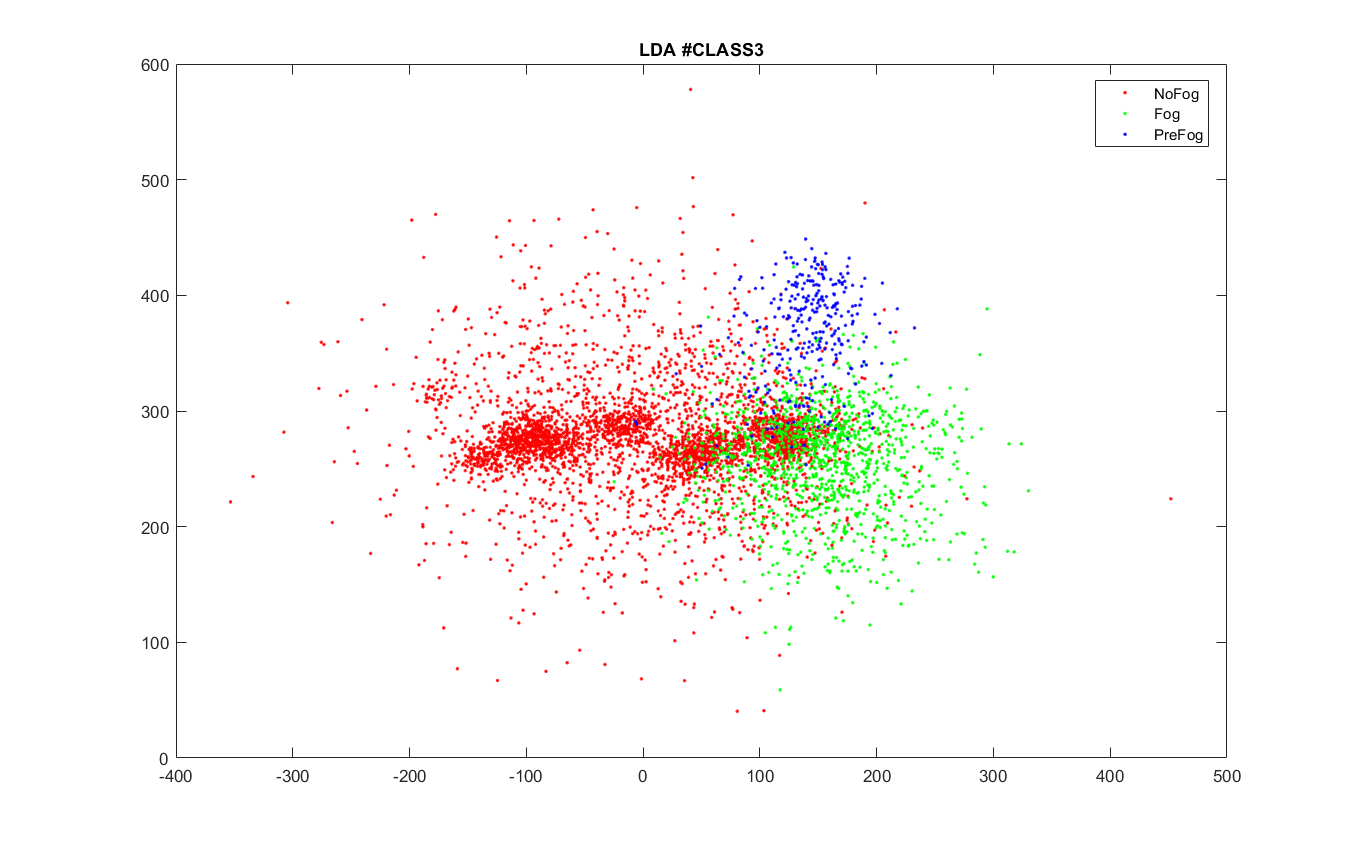
\includegraphics[scale=0.3]{images/LDAALL.png}
	\caption{Grafico delle 3 classi in base alla discriminazione dell'approccio di Fisher presi tutti i pazienti}
	\label{LDAALL}
\end{figure}
\section{Determinazione del miglior intervallo di finestra}
In letteratura, la finestra temporale su cui vengono calcolate le feature é stata presa molte volte a priori, basandosi su delle ipotesi. Non é mai stato presentato uno studio su quale possa essere il miglior intervallo di divisione dei dati per calcolare le feature. Quello che ci prefissiamo in questa sezione é dunque testare diverse combinazioni di durata delle finestre con sovrapposizione al fine di trovare quella che meglio divide i nostri dati. Allo stesso tempo, effettuiamo tale studio con l'uso di algoritmi di clustering al fine di cercare di sostituire il dottore nella fase di etichettatura dei dati.  L'approccio che è stato preso in considerazione è basato sul calcolo di feature (o proprietà) derivanti dalla matematica statistica. Il flusso di tale approccio è:
\begin{enumerate}
	\item Pre-processamento dei dati degli accelerometri, al fine di eliminare il rumore presente ed identificare eventuali punti di outline, ossia campioni che non presentano affinità col resto dei dati poiché dovuti a movimenti non consoni;
	\item Finestramento dei dati in base ad intervalli variabili al fine di calcolare le feature, dove ogni intervallo presenta una certa sovrapposizione con l'intervallo precedente;
	\item Calcolo effettivo delle feature statistiche;
	\item Applicazione degli algoritmi di clustering;
	\item Calcolo di metriche che indicano quanto bene gli algoritmi di clustering hanno diviso i dati in relazione alle label fornite dal dataset.
\end{enumerate}
\begin{figure}[h!]
	\centering
	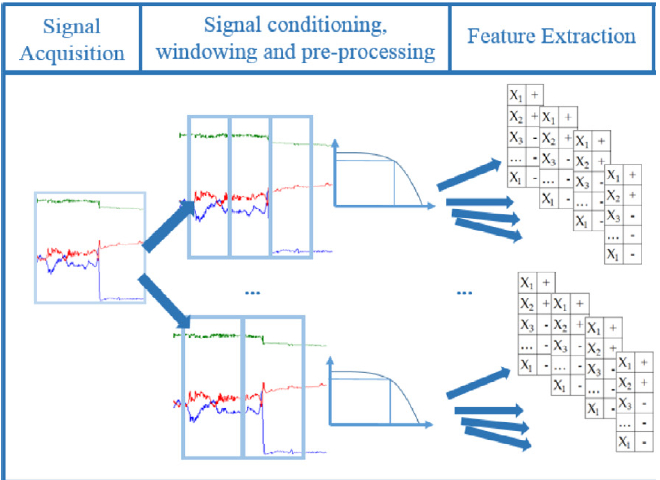
\includegraphics[scale=0.6]{images/flusso_feature.png}
	\caption{Schema generale di calcolo delle feature statistiche}
	\label{Flusso Feature}
\end{figure}
\subsection{Pre-processamento dei dati}
Gli accelerometri sono dispositivi che misurano le vibrazioni o l'accelerazione del movimento di una struttura. La forza generata dalle vibrazioni o una variazione del movimento (accelerazione) fa in modo che la massa "comprima" il materiale piezoelettrico, che genera una carica elettrica proporzionale alla forza esercitata su di esso. Dato che la carica è proporzionale alla forza e che la massa è una costante, la carica è proporzionale anche all'accelerazione. Come tutti i dispositivi che misurano delle grandezze presentano dell'incertezza strumentale che può portare ad avere rumore, ossia un segnale non desiderato, di origine naturale o artificiale, che si sovrappone all'informazione degli accelerometri stessi. Questo rumore porta ad avere dei punti definiti outlier, ossia campioni che non presentano affinità col resto dei dati poiché dovuti a movimenti non consoni.\\
Al fine di rimuovere tali punti, che altererebbero in modo negativo il calcolo delle nostre feature, si rende necessario rimuoverli dal nostro dataset. Per identificarli, è stato implementato un filtro passa-alto che eliminano tutte le frequenze inferiori a 0.5Hz, le quali non appartengono al normale movimento umano ma indicano appunto la presenza di rumore, come evidenziato in \cite{21}.
\subsection{Definizione degli intervalli}
Una volta filtrati i dati, il passo successivo dell'algoritmo consiste nel dividerli in intervalli temporali, al fine di poter computare le caratteristiche degli stessi. Un intervallo contiene un determinato movimento, che però verrebbe "interrotto" con la fine della finestra stessa e quindi potrei perdere informazioni su tale movimento. Per evitare il più possibile tale perdita, è usato usato un approccio che sfrutta le sovrapposizioni tra intervalli, per cui ogni nuova finestra non inizia subito dopo la fine della precedente, ma all'interno di essa. La durata degli intervalli che sono stati presi in considerazione sono:
\begin{itemize}
	\item  Da 1 secondi a 5 secondi per la finestra temporale, con un incremento di 0.5 secondi;
	\item Da 0.5 a 4.5 secondi per l'intervallo di overlap, con un incremento sempre di 0.5 secondi.
\end{itemize}
La condizione fondamentale per usare le sovrapposizioni è che l'intervallo delle stesse non sia mai maggiore della durata delle finestre temporali, per cui è stata posta la condizione che la finestra temporale sia sempre almeno 0.5 secondi più lunga dell'intervallo di sovrapposizione. Per capire da dove parte la nuova finestra, quindi, prendiamo la posizione a cui siamo arrivati e togliamo la durata della sovrapposizione. L'implementazione viene fornita in \ref{intervals}.
\begin{lstlisting}[style=Matlab-editor,frame=single, caption=Definizione degli intervalli, label=intervals]  % Start your code-block
...
for k = 5:5:45

Y = k/10;

for i = (Y+0.5):0.5:5
%dimensione della finestra in secondi
size_windows_sec = i;
%dimensione della finestra in campioni
size_windows_sample = Fs * i;

%dimensione dell'overlap in secondi
size_overlap_sec = Y;
%dimensione dell'overlap in campioni
size_overlap_samples = Fs * Y;

number_sample = 1;

%for each sample window, compute the features
for i=1:size_windows_sample-size_overlap_samples:m - size_windows_sample
B = A(i:i+size_windows_sample-1,:);
...
\end{lstlisting}
\subsection{Calcolo delle Feature}
 Per ogni possibile combinazione di finestra temporale e sovrapposizione, a questo punto vengono calcolate le feature per ogni intervallo. Le feature prese in considerazione nel nostro studio sono descritte in tabella \ref{TAB:Feature}.
\begin{table}[h!]
	\begin{tabular}{ |p{0.05\textwidth} | p{0.25\textwidth} | p{0.6\textwidth} | }
		\multicolumn{1}{|p{0.05\textwidth} |}{\textbf{N}} &  
		\multicolumn{1}{p{0.25\textwidth} |}{\textbf{Feature}} &
		\multicolumn{1}{p{0.6\textwidth} |}{\textbf{Descrizione}}\\
		\hline
		\hline
		1 & Minimo & Valore minimo del segnale\\
		2 & Massimo & Valore massimo del segnale \\
		3 & Mediana & Valore mediano del segnale \\
		4 & Media & Valore medio del segnale \\
		5 & Media Armonica & Media armonica del segnale \\
		6 & Errore Quadratico Medio & Valore Quadratico medio del segnale \\
		7 & Media Geometrica & Media geometrica del segnale \\
		8 & Varianza & Radice della deviazione standard \\
		9 & Deviazione Standard & Deviazione media del segnale rispetto alla media \\
		10 & Curtosi & Allontanamento dalla normalità distributiva del segnale \\
		11 & Simmetria & Grado di asimmetria della distribuzione del segnale \\
		12 & Moda & Il numero che appare più volte nel segnale \\
		13 & Media Tagliata & Media tagliatadel segnale nella finestra \\
		14 & Entropia & Misura della di distruzione delle componenti in frequenza \\
		15 & Range & Differenza tra il valore minimo e massimo del segnale \\
		16 & Magnitudine & Somma della norma euclidea di tre assi normalizzato sulla lunghezza del segnale \\
		17 & Area Magnitudine & Accelerazione della magnitudine di tre assi normalizzato sulla lunghezza del segnale \\
		18 & Autovalori delle direzioni dominanti & Autovalori della matrice di covarianza di tre assi \\
		19 & Accelerazione media dell'energia & Valore medio dell'energia sui 3 assi \\
	\end{tabular}
\caption{Descrizione delle Feature Statistiche}
\label{TAB:Feature}
\end{table}\\
Nel dataset, ogni campione è etichettato. Poiché le nostre feature sono composte da molti campioni messi assieme, si rende necessario trovare un metodo per unire, sbagliando il meno possibile, tutte le etichette della finestra che prendiamo in considerazione. Per fare ciò, si è deciso di utilizzare la funzione di moda, ossia il numero che si ripete più spesso all'interno dell'intervallo considerato. L'etichetta risultante viene inserita nella tabella e verrà utilizzata come criterio di confronto, al fine di valutare le prestazioni degli algoritmi di clustering. L'implementazione del codice è fornito in \ref{extract_feature}
\begin{lstlisting}[style=Matlab-editor,frame=single, caption=Calcolo delle Feature, label=extract_feature]  % Start your code-block
...
%time sample
F(number_sample, 1) = TIME(i,:);
%min --> minimum value for each accelerometer
F(number_sample, 2:10) = min(B);
%max --> maximum value for each accelerometer
F(number_sample, 11:19) = max(B);
%median --> median signal value
F(number_sample, 20:28) = median(B);
%mean --> average value
F(number_sample, 29:37) = mean(B);
%ArmMean --> harmonic average of the signal
F(number_sample, 38:46) = harmmean(B);
%root mean square --> quadratic mean value of the signal
F(number_sample, 47:55) = rms(B);
%variance --> square of the standard deviation
F(number_sample, 56:64) = var(B);
%standard deviation --> mean deviation of the signal compared to the
%average
F(number_sample, 65:73) = std(B);
%kurtosis --> degree of peakedness of the sensor signal distribution
%(allontanamento dalla normalita distributiva)
F(number_sample, 74:82) = kurtosis(B);
%skewdness --> degree of asymmetry of the sensor signal distribution
F(number_sample, 83:91) = skewness(B);
%mode --> number that appears most often in the signal
F(number_sample, 92:100) = mode(B);
%trim mean --> trimmed mean of the signal in the window
F(number_sample, 101:109) = trimmean(B,10);
%range --> difference between the largest and the smallest values of
%the signal
F(number_sample, 110:118) = range(B);
%signal magnitude vector --> sum of the euclidean norm over the three
%axis over the entire window normalized by the windows lenght
F(number_sample, 119) = svmn(B(:,1:3), length(B));
F(number_sample, 120) = svmn(B(:,4:6), length(B));
F(number_sample, 121) = svmn(B(:,7:9), length(B));
%normalized signal magnitude area --> acceleration magnitude summed
%over three axes normalized by the windows length
F(number_sample, 122) = sman(B(:,1:3), length(B));
F(number_sample, 123) = sman(B(:,4:6), length(B));
F(number_sample, 124) = sman(B(:,7:9), length(B));
%eigenvalues of dominant directions --> eigenvalues of the
%covariance matrix of the acceleration data along x, y and z axis
F(number_sample,125) = eigs(cov(B(:,1:3)),1);
F(number_sample,126) = eigs(cov(B(:,4:6)),1);
F(number_sample,127) = eigs(cov(B(:,7:9)),1);
%averaged acceleration energy --> mean value of the energy over
%three acceleration axes
F(number_sample,128) = energyn(B(:,1:3),length(B));
F(number_sample,129) = energyn(B(:,4:6),length(B));
F(number_sample,130) = energyn(B(:,7:9),length(B));
%is freezing?
F(number_sample,131) = mode(FREEZE(i:i+size_windows_sample-1,:));

%go to next sample
number_sample = number_sample + 1;
...
\end{lstlisting}
\subsection{Clustering}
Essendo il nuovo dataset composto dalle caratteristiche dei dati originali divisi in intervalli, si possono applicare gli algoritmi di clustering. Quelli che sono stati presi in considerazione nella nostra analisi sono: K-means, Fuzzy C-Means e Neural Network. Il K-means viene testato in 4 varianti diverse, in base alle seguenti metriche di distanza: cityblock, correlation, cosine, euclidean.\\
Ogni algoritmo di clustering viene applicato in tutte le possibili combinazioni di intervalli ed ognuno di essi restituisce un vettore di numeri, che corrispondono alle etichette che assegnano ad ogni vettore di feature. Questi vengono salvati e verranno poi utilizzati per calcolare le prestazioni degli algoritmi stessi in confronto alla classificazione originale del dottore. L'implementazione del codice è fornita in \ref{clustering}
\begin{lstlisting}[style=Matlab-editor,frame=single, caption=Uso degli algoritmi di clustering, label=clustering]  % Start your code-block
...
            %% k-means %%%

% choose of parameter
means1 = 'sqeuclidean';
means2 = 'correlation';
means3 = 'cityblock';
means4 = 'cosine';
for q=1:4
if q == 1
dist_k = means1;
end
if q == 2
dist_k = means2;
end
if q == 3
dist_k = means3;
end
if q == 4
dist_k = means4;
end
options_km = statset('UseParallel', false);
maxiter = 100000;
% cluster
kidx = kmeans(bonds, numClust, 'distance', dist_k, 'options', options_km, 'MaxIter', maxiter);

P = array2table([A(:,n) kidx]);
writetable(P, [datadir 'versus_kmeans_' dist_k '_' fileruns(r).name] );
display([datadir 'versus_kmeans_' dist_k '_' fileruns(r).name]);
end

%%% neural networks - Self organizing Maps %%%

% Create a Self-Organizing Map
dimension1 = 3;
dimension2 = 1;
net = selforgmap([dimension1 dimension2]);

% Train the network
net.trainParam.showWindow = 0;
[net,tr] = train(net,bonds');

% Test the network
nidx = net(bonds');
nidx = vec2ind(nidx)';

P = array2table([A(:,n) nidx]);
writetable(P, [datadir 'versus_net_' fileruns(r).name] );
display([datadir 'versus_net_' fileruns(r).name]);


%     %%% FUZZY C-MEANS %%%
options(1) = 2;
options(2) = 10000;
options(3) = 1e-5;
options(4) = 0;
% Hide iteration information by passing appropriate options to FCM
[centres,U] = fcm(bonds,numClust,options);
[~, fidx] = max(U);
fidx = fidx';


P = array2table([A(:,n) fidx]);
writetable(P, [datadir 'versus_cmeans_' fileruns(r).name] );
display([datadir 'versus_cmeans_' fileruns(r).name]);
...
\end{lstlisting}
\subsection{Calcolo delle prestazioni}
Ogni algoritmo di clustering, per tutte le combinazioni di finestra ed overlap, fornisce un vettore di etichette. Questo rappresenta la divisione in cluster effettuata dall'algoritmo, i quali andranno confrontati con le etichette reali del dataset. Per fare questo, procediamo al calcolo di metriche quali, in ordine, accuratezza, precisione, sensitività e F1-measure. Per quanto riguarda la precisione, la sensitività e l'F1-measure, esse sarebbero relative ad ogni classe, ma poiché ci interessa indovinare la maggior parte delle volte tutte e 3 le classi, quelle che saranno riportate sono la media dei valori per ogni classe. Il codice implementativo é fornito in \ref{rate}

\begin{lstlisting}[style=Matlab-editor,frame=single, caption=Calcolo delle prestazioni, label=rate]  % Start your code-block
...
% Matrice di confusione
[C,order] = confusionmat(D(:,2),D(:,1));
accuracy = c_accuracy(C);
precision = c_precision(C);
recall = c_recall(C);
F1measure = c_F1measure(precision,recall);

B = [accuracy precision recall F1measure];
E = [E B];

end
Q = [Q ; [e E]];
e = [e [0 0 0 0]];
...
\end{lstlisting}
Viene creata dunque una tabella che riassume, per ogni possibile intervallo, le prestazioni dell'algoritmo, come si vede in \ref{ratecluster1}, \ref{ratecluster2}, \ref{ratecluster3}.
\begin{table}[htp]
	\centering
	\caption{Esempio di tabelle delle prestazioni del clustering}
	\label{ratecluster1}
	\resizebox{\textwidth}{!}{%
	\begin{tabular}{|l|l|l|l|l|l|l|l|l|l|l|l|l|}
		\hline
		& \multicolumn{4}{c|}{Secondi: 1} & \multicolumn{4}{c|}{Secondi: 1.5} & \multicolumn{4}{c|}{Secondi: 2} \\ \hline
		Ov 0.5 & 0,7 & 0,6 & 0,3 & 0,4 & 0,8 & 0,3 & 0,3 & 0,3 & 0,91 & 0,5 & 0,5 & 0,5 \\ \hline
		Ov 1 & 0 & 0 & 0 & 0 & 0,7 & 0,3 & 0,3 & 0,3 & 0,8 & 0,6 & 0,5 & 0,55 \\ \hline
		Ov 1.5 & 0 & 0 & 0 & 0 & 0 & 0 & 0 & 0 & 0,91 & 0,72 & 0,6 & 0,6 \\ \hline
	\end{tabular}%
}
\end{table}
\begin{table}[htp]
	\centering
	\caption{Esempio di tabelle delle prestazioni del clustering}
	\label{ratecluster2}
	\resizebox{\textwidth}{!}{%
	\begin{tabular}{|l|l|l|l|l|l|l|l|l|l|l|l|l|}
		\hline
		& \multicolumn{4}{c|}{Secondi: 2.5} & \multicolumn{4}{c|}{Secondi: 3} & \multicolumn{4}{c|}{Secondi: 3.5} \\ \hline
		Ov 0.5 & 0,7 & 0,3 & 0,3 & 0,3 & 0,4 & 0,1 & 0,2 & 0,17 & 0,46 & 0,32 & 0,4 & 0,35 \\ \hline
		Ov 1 & 0,05 & 0,3 & 0,2 & 0,3 & 0,46 & 0,3 & 0,4 & 0,38 & 0,46 & 0,32 & 0,4 & 0,35 \\ \hline
		Ov 1.5 & 0,75 & 0,2 & 0,2 & 0,2 & 0,8 & 0,3 & 0,3 & 0,3 & 0,46 & 0,32 & 0,4 & 0,35 \\ \hline
		Ov 2 & 0,8 & 0,3 & 0,3 & 0,3 & 0,6 & 0,3 & 0,1 & 0,21 & 0,46 & 0,32 & 0,4 & 0,35 \\ \hline
		Ov2.5 & 0 & 0 & 0 & 0 & 0,81 & 0,26 & 0,24 & 0,25 & 0,7 & 0,3 & 0,2 & 0,26 \\ \hline
		Ov 3 & 0 & 0 & 0 & 0 & 0 & 0 & 0 & 0 & 0,6 & 0,3 & 0,31 & 0,31 \\ \hline
	\end{tabular}%
}
\end{table}
\begin{table}[htp]
	\centering
	\caption{Esempio di tabelle delle prestazioni del clustering}
	\label{ratecluster3}
	\resizebox{\textwidth}{!}{%
	\begin{tabular}{|l|l|l|l|l|l|l|l|l|l|l|l|l|}
		\hline
		& \multicolumn{4}{c|}{Secondi: 4} & \multicolumn{4}{c|}{Secondi: 4.5} & \multicolumn{4}{c|}{Secondi: 5} \\ \hline
		Ov 0.5 & 0,8 & 0,36 & 0,35 & 0,35 & 0,81 & 0,32 & 0,34 & 0,33 & 0,75 & 0,24 & 0,26 & 0,25 \\ \hline
		Ov 1 & 0,76 & 0,21 & 0,28 & 0,26 & 0,79 & 0,32 & 0,34 & 0,31 & 0,79 & 0,3 & 0,3 & 0,3 \\ \hline
		Ov 1.5 & 0,46 & 0,36 & 0,33 & 0,35 & 0,8 & 0,36 & 0,35 & 0,35 & 0,59 & 0,24 & 0,33 & 0,29 \\ \hline
		Ov 2 & 0,41 & 0,33 & 0,44 & 0,39 & 0,76 & 0,21 & 0,28 & 0,26 & 0,26 & 0,79 & 0,32 & 0,34 \\ \hline
		Ov2.5 & 0,59 & 0,24 & 0,33 & 0,29 & 0,46 & 0,36 & 0,33 & 0,35 & 0,35 & 0,8 & 0,36 & 0,35 \\ \hline
		Ov 3 & 0,44 & 0,11 & 0,12 & 0,11 & 0,41 & 0,33 & 0,44 & 0,39 & 0,8 & 0,36 & 0,35 & 0,35 \\ \hline
		Ov 3.5 & 0,78 & 0,23 & 0,33 & 0,28 & 0,75 & 0,24 & 0,26 & 0,25 & 0,76 & 0,21 & 0,28 & 0,26 \\ \hline
		Ov 4 & 0 & 0 & 0 & 0 & 0,79 & 0,3 & 0,3 & 0,3 & 0,75 & 0,24 & 0,26 & 0,25 \\ \hline
		Ov 4.5 & 0 & 0 & 0 & 0 & 0 & 0 & 0 & 0 & 0,79 & 0,3 & 0,3 & 0,3 \\ \hline
	\end{tabular}%
	}
\end{table}
\subsection{Risultati Clustering}
Dopo che sono state generate tutte le tabelle per tutti i pazienti in cui vengono espressi i valori di accuratezza, precisione, sensitività e F1-measure, siamo interessati all'intervallo migliore, ossia quello che ci fornisce i valori maggiori delle metriche suddette. Per fare questo, analizziamo ogni tabella e, per ogni algoritmo, salviamo l'intervallo ed i valori che presentano le metriche migliori, come nel caso delle tabelle \ref{ratecmeans}, \ref{ratekmeans}, \ref{rateneuralnetwork}. La metrica riportata per il k means é la square euclidean, in quanto é quella che ci ha portato ad i risultati migliori. \\
Ogni tabella descrive:
\begin{itemize}
	\item l'algoritmo di clustering che é stato utilizzato;
	\item il paziente del test;
	\item i valori delle metriche migliori trovate;
	\item la combinazione overlap-secondi in cui risultano tali metriche.
\end{itemize}

% Please add the following required packages to your document preamble:
% \usepackage{graphicx}
\begin{table}[]
	\centering
	\caption{Rate Pazienti per l'algoritmo di clustering C-means}
	\label{ratecmeans}
	\resizebox{\textwidth}{!}{%
		\begin{tabular}{|l|l|l|l|l|l|l|}
			\hline
			\textbf{}         & \multicolumn{6}{c|}{\textbf{CMEANS}}                                                                              \\ \hline
			\textbf{Paziente} & \textbf{Accuratezza} & \textbf{Precisione} & \textbf{Recall} & \textbf{F1} & \textbf{Overlap} & \textbf{Finestra} \\ \hline
			\textbf{S01}      & 0,92                 & 0,31                & 0,33            & 0,32        & 1                & 2                 \\ \hline
			\textbf{S02}      & 0,44                 & 0,46                & 0,63            & 0,53        & 1                & 2                 \\ \hline
			\textbf{S03}      & 0,7                  & 0,51                & 0,57            & 0,54        & 1                & 2                 \\ \hline
			\textbf{S04}      & 0,7                  & 0,33                & 0               & 0           & 0,5                & 1               \\ \hline
			\textbf{S05}      & 0,53                 & 0,49                & 0,46            & 0,47        & 1                & 1,5               \\ \hline
			\textbf{S06}      & 0,57                 & 0,36                & 0,32            & 0,34        & 1                & 1,5               \\ \hline
			\textbf{S07}      & 0,48                 & 0,37                & 0,43            & 0,4         & 1                & 1,5               \\ \hline
			\textbf{S08}      & 0,41                 & 0,39                & 0,43            & 0,41        & 1,5              & 2                 \\ \hline
			\textbf{S09}      & 0,59                 & 0,35                & 0,37            & 0,36        & 1                & 1,5               \\ \hline
			\textbf{S10}      & 0,73                 & 0,33                & 0               & 0           & 0,5                & 1               \\ \hline
		\end{tabular}%
	}
\end{table}

% Please add the following required packages to your document preamble:
% \usepackage{graphicx}
\begin{table}[]
	\centering
	\caption{Rate Pazienti per l'algoritmo di clustering K-means}
	\label{ratekmeans}
	\resizebox{\textwidth}{!}{%
		\begin{tabular}{|l|l|l|l|l|l|l|}
			\hline
			\textbf{Tutti}    & \multicolumn{6}{c|}{\textbf{KMEANS}}                                                                              \\ \hline
			\textbf{Paziente} & \textbf{Accuratezza} & \textbf{Precisione} & \textbf{Recall} & \textbf{F1} & \textbf{Overlap} & \textbf{Finestra} \\ \hline
			\textbf{S01}      & 0,92                 & 0,72                & 0,34            & 0,46        & 1,5              & 2                 \\ \hline
			\textbf{S02}      & 0,82                 & 0,61                & 0,34            & 0,44        & 1                & 2                 \\ \hline
			\textbf{S03}      & 0,75                 & 0,78                & 0,54            & 0,64        & 1,5              & 2                 \\ \hline
			\textbf{S04}      & 1                    & 0,33                & 0               & 0           & 0,5                & 1               \\ \hline
			\textbf{S05}      & 0,67                 & 0,56                & 0,33            & 0,42        & 1                & 2                 \\ \hline
			\textbf{S06}      & 0,91                 & 0,3                 & 0,33            & 0,32        & 1                & 1,5               \\ \hline
			\textbf{S07}      & 0,92                 & 0,31                & 0,33            & 0,32        & 1                & 2                 \\ \hline
			\textbf{S08}      & 0,7                  & 0,57                & 0,34            & 0,42        & 1                & 1,5               \\ \hline
			\textbf{S09}      & 0,81                 & 0,6                 & 0,34            & 0,43        & 1                & 2                 \\ \hline
			\textbf{S10}      & 1                    & 0,33                & 0               & 0           & 0,5                & 1,5               \\ \hline
		\end{tabular}%
	}
\end{table}

% Please add the following required packages to your document preamble:
% \usepackage{graphicx}
\begin{table}[]
	\centering
	\caption{Rate Pazienti per l'algoritmo di clustering Self-Organizing Map}
	\label{rateneuralnetwork}
	\resizebox{\textwidth}{!}{%
		\begin{tabular}{|l|l|l|l|l|l|l|}
			\hline
			\textbf{Tutti}    & \multicolumn{6}{c|}{\textbf{NEURAL NETWORK}}                                                                      \\ \hline
			\textbf{Paziente} & \textbf{Accuratezza} & \textbf{Precisione} & \textbf{Recall} & \textbf{F1} & \textbf{Overlap} & \textbf{Finestra} \\ \hline
			\textbf{S01}      & 0,92                 & 0,31                & 0,33            & 0,32        & 1                & 1,5               \\ \hline
			\textbf{S02}      & 0,81                 & 0,44                & 0,34            & 0,38        & 1                & 1,5               \\ \hline
			\textbf{S03}      & 0,75                 & 0,78                & 0,54            & 0,63        & 1                & 2                 \\ \hline
			\textbf{S04}      & 0,64                 & 0,33                & 0               & 0           & 0,5                & 1                 \\ \hline
			\textbf{S05}      & 0,58                 & 0,42                & 0,46            & 0,44        & 1                & 2                 \\ \hline
			\textbf{S06}      & 0,57                 & 0,32                & 0,31            & 0,31        & 1                & 1,5               \\ \hline
			\textbf{S07}      & 0,63                 & 0,3                 & 0,26            & 0,28        & 1                & 2                 \\ \hline
			\textbf{S08}      & 0,56                 & 0,69                & 0,38            & 0,49        & 1,5              & 2                 \\ \hline
			\textbf{S09}      & 0,57                 & 0,37                & 0,41            & 0,39        & 1                & 2                 \\ \hline
			\textbf{S10}      & 1                    & 0,33                & 0               & 0           & 0,5                & 1               \\ \hline
		\end{tabular}%
	}
\end{table}
\subsection{LDA con intervallo migliore}
In \ref{LDAS01} e \ref{LDAS02} si era notato come esiste una certa distinzione tra le classi, ma c'era una sovrapposizione tra alcuni dati di esse, il che ci porta a studiare quale sia il miglior intervallo di divisione dei dati. Analogamente al procedimento per la fase di clustering, iteriamo l'algoritmo di LDA cambiando la durata della finestra temporale e la sovrapposizione tra di essi. Gli intervalli possibili, come nel caso del clustering, vanno da 1 a 5 secondi per la finestra, da 0.5 a 4.5 secondi per la sovrapposizione.\\
Dopo aver provato tutte le possibili combinazioni, risulta anche in questo caso che scegliendo 2 secondi di finestra e 1 secondo di overlap si ottiene una divisione molto più netta per il singolo paziente, come si può vedere in \ref{LDAS01_best.png} e \ref{LDAS02_best.png}.\\
Anche usando i dati di tutti i pazienti si può notare, in figura \ref{LDAALL2.png}, che c'è un miglioramento nella divisione dei dati usando un intervallo di 2 secondi per la finestra ed 1 secondo per l'overlap.
\begin{figure}[]
	\centering
	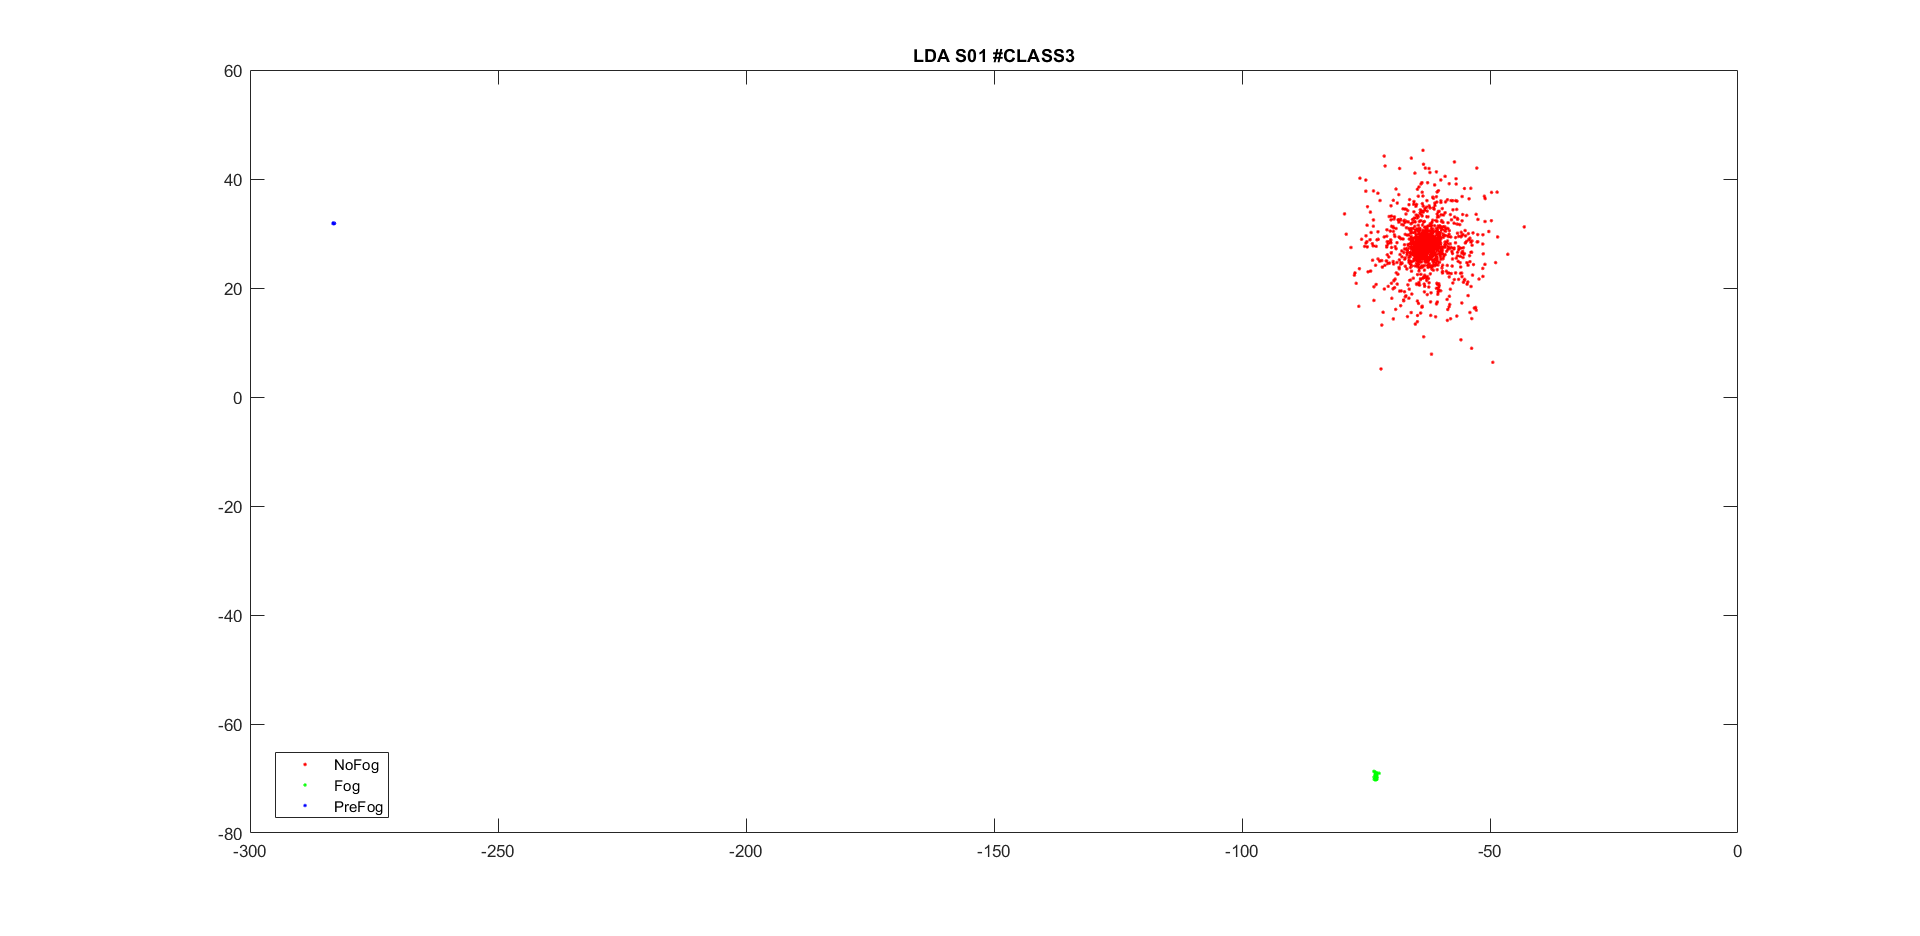
\includegraphics[scale=0.25]{images/LDAS01_best.png}
	\caption{Grafico delle 3 classi in base alla discriminazione dell'approccio di Fisher per il paziente 1 con 2 secondi di finestra ed 1 secondo di overlap}
	\label{LDAS01_best.png}
\end{figure}
\begin{figure}[]
	\centering
	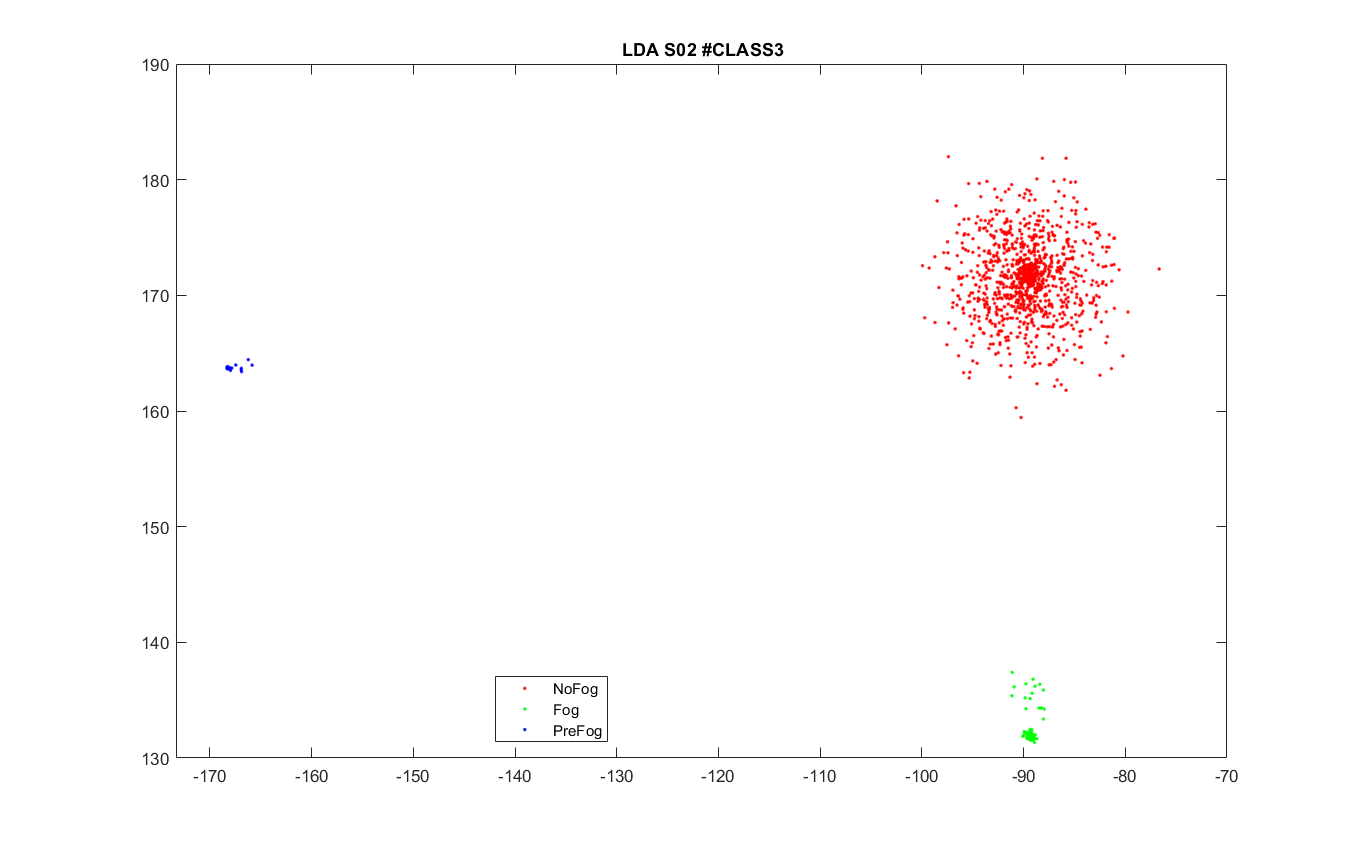
\includegraphics[scale=0.3]{images/LDAS02_best.png}
	\caption{Grafico delle 3 classi in base alla discriminazione dell'approccio di Fisher per il paziente 2 con 2 secondi di finestra ed 1 secondo di overlap}
	\label{LDAS02_best.png}
\end{figure}
\begin{figure}[]
	\centering
	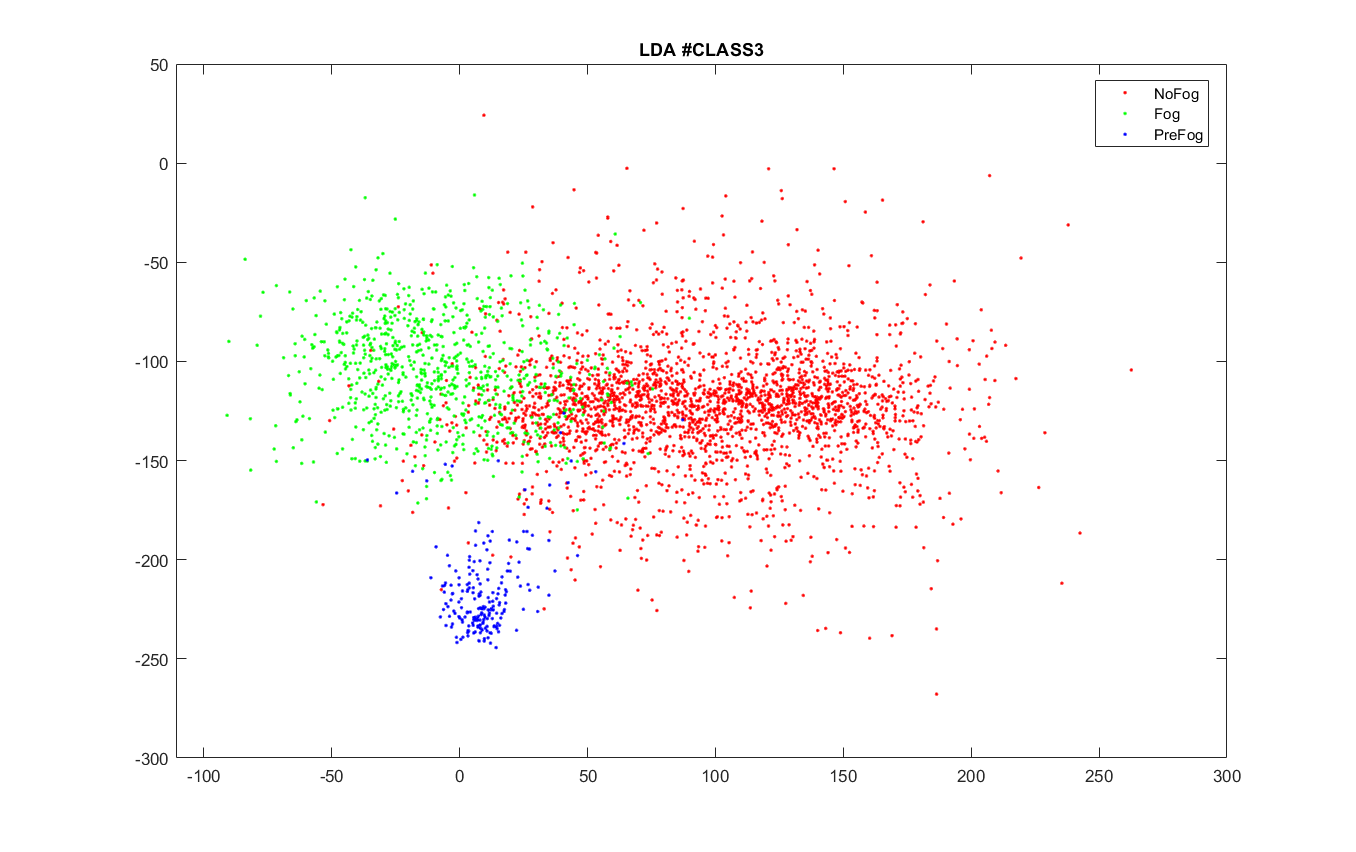
\includegraphics[scale=0.3]{images/LDAALL2.png}
	\caption{Grafico delle 3 classi in base alla discriminazione dell'approccio di Fisher per tutti i pazienti con 2 secondi di finestra ed 1 secondo di overlap}
	\label{LDAALL2.png}
\end{figure}

\subsection{Risultati}
Osservando le tabelle, si nota come il valore di overlap e dimensione della finestra che più frequentemente mi portano ad avere metriche migliori sono:
\begin{itemize}
	\item 1 secondo di sovrapposizione e 2 secondi di finestra;
	\item 1 secondo di sovrapposizione e 1,5 secondi di finestra.
\end{itemize}
L'obiettivo di sostituire il dottore nella prima fase di test, ossia raccogliere dati dagli accelerometri ed applicare le etichette di noFoG, FoG o preFoG, sembra fattibile, in quanto in molti casi abbiamo un'accuratezza superiore al 70\%, per cui nella maggior parte dei casi il clustering segna l'etichetta come corretta.\\
Il nostro studio degli intervalli, sia per la parte di clustering che per la parte di LDA, ci porta a concludere che il miglior modo con cui si possono dividere i dati in finestre per calcolare le feature é scegliere 1 secondo di sovrapposizione tra le finestre e 1,5 o 2 secondi per quanto riguarda la lunghezza della finestra temporale.

\section{Primo approccio di classificazione}
Nella sezione precedente, è stato decritto uno studio degli intervalli temporali che ci ha portati a decidere quale sia la migliore scelta di durata sia per la finestra che per la sovrapposizione al fine di dividere al meglio i dati a nostra disposizione. Dalla figura \ref{LDAALL2.png}, si nota come le classi FoG e NoFoG sono a volte confuse tra di loro, mentre il preFoG è meno confuso nelle altre due classi. Ma quest'ultima classe è proprio quella che stiamo studiando ed è quella che ci porterebbe a prevenire le occorrenze di FoG, in quanto, identificandola, avrei il tempo di dare lo stimolo prima dell'avvenuta del FoG, mentre se cerco di identificare solo i Freezing darei lo stimolo uditorio in ritardo in ogni caso. Questo ci porta a provare un primo approccio di classificazione a 2 classi, dove raggruppiamo assieme i dati di FoG e noFoG e teniamo separate le occorrenze di preFoG. L'algoritmo che è stato scelto è il K-nearest Neighbours (KNN), spiegato nel capitolo \ref{chap3:background}. Usiamo sempre l'intervallo che è stato dimostrato nella sezione precedente essere quello più affidabile. L'algoritmo verrà testato in due modi:
\begin{itemize}
	\item alleniamo il knn su un paziente singolo, effettuiamo una cross-validation sul classificatore e lo testiamo su dei nuovi dati, ossia che non sono stati inclusi nella  cross-validation;
	\item alleniamo il knn sui dati di tutti i pazienti contemporaneamente ed effettuiamo una cross-validation.
\end{itemize}
La cross-validation è una tecnica statistica utilizzabile in presenza di una buona numerosità del campione osservato o training set. In particolare la k-fold cross-validation consiste nella suddivisione del dataset totale in k parti di uguale numerosità (si chiama anche k-fold validation) e, ad ogni passo, la k-esima parte del dataset viene ad essere il validation dataset, mentre la restante parte costituisce il training dataset. In altre parole, si suddivide il campione osservato in gruppi di egual numerosità, si esclude iterativamente un gruppo alla volta e lo si cerca di predire con i gruppi non esclusi.\\
\subsection{Risultati sul singolo paziente}
Per ogni paziente su cui è stata effettuata la prova, abbiamo ricavato la media delle matrici di confusione della cross-validation. Successivamente, prendendo un altro dataset dello stesso paziente, utilizzando il knn allenato abbiamo cercato di predirre le classi del secondo dataset. Poiché non tutti i pazienti presentano, nel dataset, due diversi file (ossia due prove di camminata), la prova è stata possibile solo su alcuni di essi.\\
In tabella \ref{MCcross1} possiamo osservare le matrici di confusione della cross-validation a 10 gruppi per i pazienti numero 1, 2, 3, 5, 7, ossia quelli con doppio file. Si può notare come la matrice risulti diagonali, il che vuole dire che etichetta, nella cross-validation, sempre giusti i nostri campioni sullo stesso paziente.\\
In tabella \ref{MCprev1}, ossia quella relativa alla predizione su un nuovo file, osserviamo che la matrice è abbastanza più confusa, per cui alcune volte etichetta occorrenze di preFoG come altro e non casi di preFoG come preFog. In tabella \ref{Mpred} si possono osservare le metriche di accuracy, sensitivity, specificity ed F1-measure per la predizione. Questo risultato può essere dato dal fatto che, anche per lo stesso paziente, percorsi diversi o situazioni diverse portano ad una camminata differente da quelle precedenti, e quindi ho dati che possono risultare molto simili ma appartenere a casi diversi nei due test.\\
La cross-validation restituisce delle metriche perfette, quindi l'algoritmo riesce a classificare molto bene i punti di un dataset anche allenandosi solo su una parte di esso e prevedendo i dati esclusi. Il caso della previsione su dati di file diversi, invece, è  da migliorare, in quanto restituisce una specificità bassa, ossia tende a confondere preFoG in NoFoG o FoG. Questo fatto può essere dovuto al fatto che i movimenti, e quindi i dati, di preFoG sono altamente soggettivi e dipendenti dalla situazione in cui il paziente si trova, quindi un movimento nuovo può essere classificato male rispetto al dataset di training. Una soluzione a questo problema sarebbe quello di ottenere dei dataset più grandi, in modo tale da avere un maggior numero di movimenti su cui allenare il classificatore.
% Please add the following required packages to your document preamble:
% \usepackage{multirow}
% \usepackage{graphicx}
\begin{table}[]
	\centering
	\caption{Matrici di confusione per la cross-validation del singolo paziente}
	\label{MCcross1}
	\resizebox{\textwidth}{!}{%
		\begin{tabular}{|c|l|c|c|c|c|c|c|c|c|c|c|}
			\hline
			\textbf{Paziente}                                                                       &                & \textbf{01}                       & \textbf{}                        & \multicolumn{2}{c|}{\textbf{02}}                                     & \multicolumn{2}{c|}{\textbf{03}}                                     & \multicolumn{2}{c|}{\textbf{05}}                                     & \multicolumn{2}{c|}{\textbf{07}}                                     \\ \hline
			\multicolumn{1}{|l|}{}                                                                  & \textbf{Label} & \multicolumn{1}{l|}{\textbf{NPF}} & \multicolumn{1}{l|}{\textbf{PF}} & \multicolumn{1}{l|}{\textbf{NPF}} & \multicolumn{1}{l|}{\textbf{PF}} & \multicolumn{1}{l|}{\textbf{NPF}} & \multicolumn{1}{l|}{\textbf{PF}} & \multicolumn{1}{l|}{\textbf{NPF}} & \multicolumn{1}{l|}{\textbf{PF}} & \multicolumn{1}{l|}{\textbf{NPF}} & \multicolumn{1}{l|}{\textbf{PF}} \\ \hline
			\multirow{2}{*}{\textbf{\begin{tabular}[c]{@{}c@{}}Matrice \\ Confusione\end{tabular}}} & \textbf{NPF}   & 1413                              & 0                                & 431                               & 0                                & 1335                              & 0                                & 983                               & 0                                & 1127                              & 0                                \\ \cline{2-12} 
			& \textbf{PF}    & 0                                 & 36                               & 0                                 & 18                               & 0                                 & 84                               & 0                                 & 76                               & 0                                 & 32                               \\ \hline
		\end{tabular}%
	}
\end{table}
% Please add the following required packages to your document preamble:
% \usepackage{multirow}
% \usepackage{graphicx}
\begin{table}[]
	\centering
	\caption{Matrici di confusione per la previsione del singolo paziente}
	\label{MCprev1}
	\resizebox{\textwidth}{!}{%
		\begin{tabular}{|c|l|c|c|c|c|c|c|c|c|c|c|}
			\hline
			\textbf{Paziente}                                                                       &                & \textbf{01}                       & \textbf{}                        & \multicolumn{2}{c|}{\textbf{02}}                                     & \multicolumn{2}{c|}{\textbf{03}}                                     & \multicolumn{2}{c|}{\textbf{05}}                                     & \multicolumn{2}{c|}{\textbf{07}}                                     \\ \hline
			\multicolumn{1}{|l|}{}                                                                  & \textbf{Label} & \multicolumn{1}{l|}{\textbf{NPF}} & \multicolumn{1}{l|}{\textbf{PF}} & \multicolumn{1}{l|}{\textbf{NPF}} & \multicolumn{1}{l|}{\textbf{PF}} & \multicolumn{1}{l|}{\textbf{NPF}} & \multicolumn{1}{l|}{\textbf{PF}} & \multicolumn{1}{l|}{\textbf{NPF}} & \multicolumn{1}{l|}{\textbf{PF}} & \multicolumn{1}{l|}{\textbf{NPF}} & \multicolumn{1}{l|}{\textbf{PF}} \\ \hline
			\multirow{2}{*}{\textbf{\begin{tabular}[c]{@{}c@{}}Matrice \\ Confusione\end{tabular}}} & \textbf{NPF}   & 412                               & 27                               & 808                               & 173                              & 229                               & 20                               & 621                               & 354                              & 343                               & 90                               \\ \cline{2-12} 
			& \textbf{PF}    & 9                                 & 1                                & 23                                & 10                               & 9                                 & 1                                & 40                                & 14                               & 11                                & 5                                \\ \hline
		\end{tabular}%
	}
\end{table}

% Please add the following required packages to your document preamble:
% \usepackage{graphicx}
\begin{table}[]
	\centering
	\caption{Metriche di misura della predizione per il singolo paziente}
	\label{Mpred}
	\resizebox{\textwidth}{!}{%
		\begin{tabular}{|c|c|c|c|c|}
			\hline
			\multicolumn{1}{|l|}{\textbf{Paziente}} & \multicolumn{1}{l|}{\textbf{Accuracy}} & \multicolumn{1}{l|}{\textbf{Sensitivity}} & \multicolumn{1}{l|}{\textbf{Specificity}} & \multicolumn{1}{l|}{\textbf{F1-measure}} \\ \hline
			\textbf{S01}                            & 0.9198                                 & 0.9385                                    & 0.1000                                    & 0.9581                                   \\ \hline
			\textbf{S02}                            & 0.8067                                 & 0.8236                                    & 0.3030                                    & 0.8918                                   \\ \hline
			\textbf{S03}                            & 0.8880                                 & 0.9197                                    & 0.1000                                    & 0.9404                                   \\ \hline
			\textbf{S05}                            & 0.6171                                 & 0.6369                                    & 0.2593                                    & 0.7591                                   \\ \hline
			\textbf{S07}                            & 0.7751                                 & 0.7921                                    & 0.3125                                    & 0.8716                                   \\ \hline
		\end{tabular}%
	}
\end{table}

\subsection{Risultati usando i dati di tutti i pazienti}
Andando ad usare i dati provenienti da tutti i pazienti, si può osservare in tabella \ref{MCall}, che rappresenta la media delle matrici di confusione della cross-validation e le metriche di accuracy, sensitivity, specificity e F1-measure, come la matrice di confusione non sia diagonale come nel caso del paziente singolo, in quanto pazienti diversi hanno modi di camminare differenti e quindi porta ad avere dati diversi, i quali possono essere classificati nel modo sbagliato. Le metriche comunque sono molto buone, quindi possiamo dire che molti movimenti di preFoG sono comuni e quindi si può procedere con un modello futuro di previsione di nuovi dati, magari avendo a disposizione dei dataset più grandi e con un numero maggiore di pazienti.
\begin{table}[]
	\centering
	\caption{Matrice confusione e metriche di misura della cross-validation con i dati di tutti i pazienti}
	\label{MCall}
	\resizebox{\textwidth}{!}{%
		\begin{tabular}{|c|l|c|c|c|c|c|c|}
			\hline
			\multicolumn{1}{|l|}{}                                                                  & \textbf{Label} & \multicolumn{1}{l|}{\textbf{NPF}} & \multicolumn{1}{l|}{\textbf{PF}} & \multicolumn{1}{l|}{\textbf{Accuracy}} & \multicolumn{1}{l|}{\textbf{Sensitivity}} & \multicolumn{1}{l|}{\textbf{Specificity}} & \multicolumn{1}{l|}{\textbf{F1-measure}} \\ \hline
			\multirow{2}{*}{\textbf{\begin{tabular}[c]{@{}c@{}}Matrice \\ Confusione\end{tabular}}} & \textbf{NPF}   & 8426                              & 898                              & 0.90                                   & 0.90                                    & 0.89                                 & 0.95                                     \\ \cline{2-8} 
			& \textbf{PF}    & 39                                & 309                              &                                        &                                         &                                      &                                          \\ \hline
		\end{tabular}%
	}
\end{table}